\documentclass[xcolor=svgnames,14pt]{beamer}
\usepackage[utf8]{inputenc}
\usepackage{bbding,verbatim,graphicx}
\usetheme{Parasim}

\newcounter{drawings}
\newcommand{\draw}{\structure{\PencilRightDown\stepcounter{drawings}\arabic{drawings}}}
\newcommand{\qmodels}{\models\hspace{-1.7ex}\raisebox{2.7mm}{\scriptsize?}\hspace{1ex}}

\title[Parasim]{Tool for Parallel Simulations and Verification}
\author{Jan Papou\v{s}ek, Tom\'{a}\v{s} Vejpustek}
\institute{}
\date{10 May 2013}

\begin{document}

\frame[plain]{\titlepage}

\begin{frame}{Parasim}%{{{
	\begin{itemize}
		\item tool for parallel simulations and verification
		\item Java-based, open source, freeware
		\item contributors: Sven, Papi, Tom\'{a}\v{s}
		\item available on \mbox{\url{https://github.com/sybila/parasim/wiki}}
	\end{itemize}
\end{frame}%}}}
\begin{frame}{Milestones}%{{{
	\begin{itemize}
		\setlength\itemindent{20mm}
		\item[Start of 2012] Program for Support of Students' Projects
		\item[Summer 2012] Working CLI application
		\item[Autumn 2012] GUI application, user documentation
		\item[Spring 2013] Acceleration, extensions
	\end{itemize}
\end{frame}%}}}
\begin{frame}{Outline}%{{{
	\begin{enumerate}
		\item continuous deterministic systems verification
		\item how Parasim does this
		\item Parasim structure
		\item analysis demonstration
	\end{enumerate}
\end{frame}%}}}
\begin{frame}{Goal}%{{{
	$$\mathcal{M}\qmodels\varphi$$
	\begin{itemize}
		\item automatic deciding procedure
		\item feasible for \emph{discrete} systems
		\item difficult for \emph{continuous} systems
	\end{itemize}
\end{frame}%}}}
\begin{frame}{Setting}%{{{
	\begin{itemize}
		\setlength\itemindent{15mm}
		\item[model] system of ordinary differential equations
		\item[parameters] initial conditions, coefficients
		\item simulation $\implies$ trajectories
		\item[property] temporal logic formula
		\item monitoring: $s\qmodels\varphi$
	\end{itemize}
\end{frame}%}}}
\begin{frame}{Perturbation Set}%{{{
	\begin{itemize}
		\item hyperrectangle in parameter space
			\begin{center}$P:p_1\in[a_1,b_1], p_2\in[a_2,b_2],\ldots,p_n\in[a_n,b_n]$\end{center}
		\item satisfaction set -- set of parameter values which
			generate trajectories satisfying $\varphi$ \draw
		\item property satisfaction w.r.t. perturbation set
			\begin{center}$P\qmodels\phi$\end{center}
			$\forall$, proportion, sets
	\end{itemize}
\end{frame}%}}}
\begin{frame}{Satisfaction w.r.t Perturbation Set}%{{{
	\begin{itemize}
		\item continous set $\implies$ infinitely many points
		\item approximation -- efficient, reasonably precise
		\item[$\implies$] sampling (representants) \draw
			\begin{itemize}
				\item random
				\item dense
			\end{itemize}
		\item dimensionality curse -- $n^d$ samples
		\item[$\implies$] intelligent exploration
	\end{itemize}
\end{frame}%}}}
\begin{frame}{Robustness}%{{{
	\begin{center}$\rho(\varphi,s)$\end{center}
	\begin{itemize}
		\item robust signal neighbourhood -- tube
		\item how much $s$ can deviate while satisfying $\phi$
	\end{itemize}
	\begin{center}$d(s,s')\le|\rho(\varphi,s)|\implies(s\models\varphi\iff s'\models\varphi)$\end{center}
\end{frame}%}}}
\begin{frame}{Robust Neighbourhood}%{{{
	\begin{center}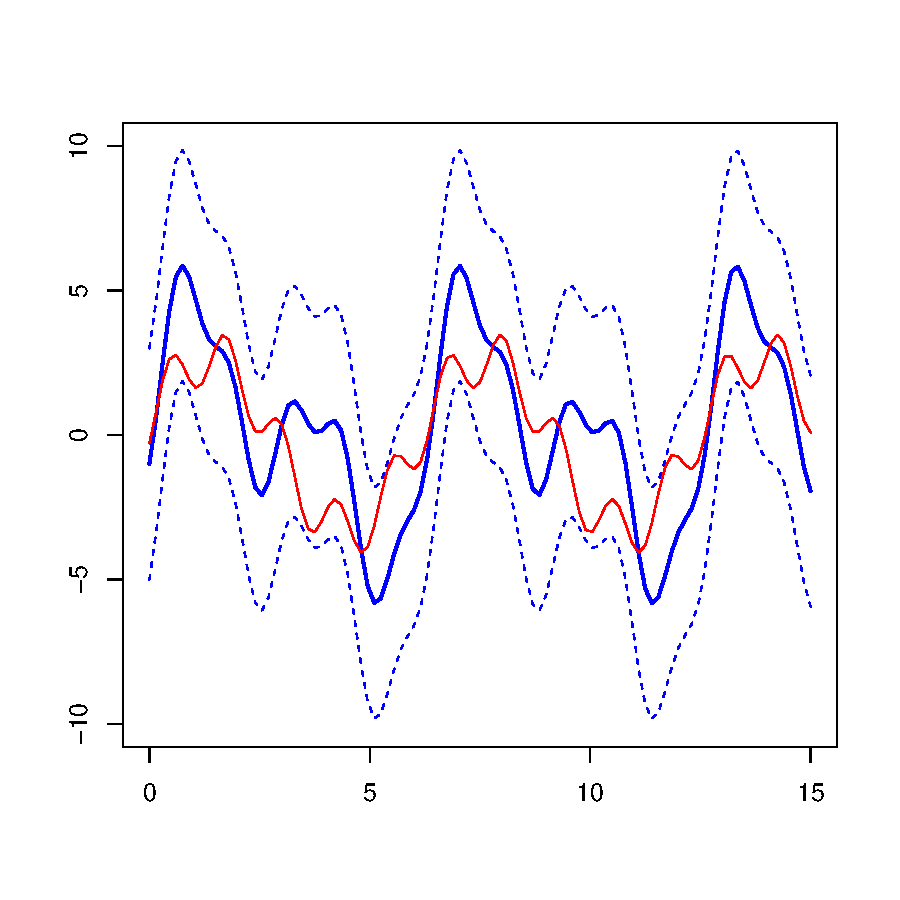
\includegraphics[width=0.7\textwidth]{tube.pdf}\end{center}
\end{frame}%}}}
\begin{frame}{Parasim Heuristics}%{{{
	\begin{itemize}
		\item signal neighbourhood $\approx$ parameter space neighbourhood
		\item movement in parameter space does not change signals too much \draw
		\item samples are chosen according to robustness
	\end{itemize}
\end{frame}%}}}
\end{document}
